%%%%%%%%%%%%%%%%%%%%%%%%%%%%%%%%%%%%%%%%%%%%%%%%%%%%%%%%%%%%%%%%%
% MUW Presentation
% LaTeX Template
% Version 1.0 (27/12/2016)
%
% License:
% CC BY-NC-SA 4.0 (http://creativecommons.org/licenses/by-nc-sa/3.0/)
%
% Created by:
% Nicolas Ballarini, CeMSIIS, Medical University of Vienna
% nicoballarini@gmail.com
% http://statistics.msi.meduniwien.ac.at/
%
% Customized for UAH by:
% David F. Barrero, Departamento de Automática, UAH
%%%%%%%%%%%%%%%%%%%%%%%%%%%%%%%%%%%%%%%%%%%%%%%%%%%%%%%%%%%%%%%%%

\documentclass[10pt,compress]{beamer} % Change 10pt to make fonts of a different size
\mode<presentation>

\usepackage[spanish]{babel}
\usepackage{fontspec}
\usepackage{tikz}
\usepackage{etoolbox}
\usepackage{xcolor}
\usepackage{xstring}
\usepackage{listings}

% Introduced by David
\usepackage{eurosym}

\usetheme{UAH}
\usecolortheme{UAH}
\setbeamertemplate{navigation symbols}{} 
\setbeamertemplate{caption}[numbered]

%%%%%%%%%%%%%%%%%%%%%%%%%%%%%%%%%%%%%%%%%%%%%%%%%%%%%%%%%%%%%%%%%
%% Presentation Info
\title[Design patterns in videogames]{Design patterns in videogames}
\author{}
\institute{\asignatura}
\date{}
%%%%%%%%%%%%%%%%%%%%%%%%%%%%%%%%%%%%%%%%%%%%%%%%%%%%%%%%%%%%%%%%%


%%%%%%%%%%%%%%%%%%%%%%%%%%%%%%%%%%%%%%%%%%%%%%%%%%%%%%%%%%%%%%%%%
%% Descomentar para habilitar barra de navegación superior
\ponerNavegacion
%%%%%%%%%%%%%%%%%%%%%%%%%%%%%%%%%%%%%%%%%%%%%%%%%%%%%%%%%%%%%%%%%

%%%%%%%%%%%%%%%%%%%%%%%%%%%%%%%%%%%%%%%%%%%%%%%%%%%%%%%%%%%%%%%%%
%% Configuración de logotipos en portada
%% Opacidad de los logotipos
\newcommand{\opacidad}{1}
%% Descomentar para habilitar logotipo en pié de página de portada
\renewcommand{\logoUno}{Images/isg.png}
%% Descomentar para habilitar logotipo en pié de página de portada
%\renewcommand{\logoDos}{Images/CCLogo.png}
%% Descomentar para habilitar logotipo en pié de página de portada
%\renewcommand{\logoTres}{Images/ALogo.png}
%% Descomentar para habilitar logotipo en pié de página de portada
%\renewcommand{\logoCuatro}{Images/ELogo.png}
%%%%%%%%%%%%%%%%%%%%%%%%%%%%%%%%%%%%%%%%%%%%%%%%%%%%%%%%%%%%%%%%%

%%%%%%%%%%%%%%%%%%%%%%%%%%%%%%%%%%%%%%%%%%%%%%%%%%%%%%%%%%%%%%%%%
%% FOOTLINE
%% Comment/Uncomment the following blocks to modify the footline
%% content in the body slides. 


%% Option A: Title and institute
\footlineA
%% Option B: Author and institute
%\footlineB
%% Option C: Title, Author and institute
%\footlineC
%%%%%%%%%%%%%%%%%%%%%%%%%%%%%%%%%%%%%%%%%%%%%%%%%%%%%%%%%%%%%%%%%

\begin{document}

%%%%%%%%%%%%%%%%%%%%%%%%%%%%%%%%%%%%%%%%%%%%%%%%%%%%%%%%%%%%%%%%%
% Use this block for a blue title slide with modified footline
{\titlepageBlue
    \setbeamertemplate{headline}{}
	\setbeamercolor{frametitle}{bg=black}
	\setbeamercolor{normal text}{bg=black}
    \begin{frame}
        \titlepage
    \end{frame}
}

\begin{frame}[plain]{}
   \begin{block}{Objectives}
   \begin{itemize}
        \item Understand the need of design patterns
		\item Distinguish the main design patterns categories
		\item Apply the main patterns to problems in videogames
	\end{itemize}
	\end{block}

   \begin{block}{Bibliography}
      \begin{enumerate}
          \item  \textit{Desarrollo de Videojuegos, Arquitectura del Motor de Vieojuegos}. UCLM.
		  \item Wikipedia
      \end{enumerate} 
   \end{block}
\end{frame}

{
\eliminarNavegacion
\begin{frame}[shrink]{Table of Contents}
 \frametitle{Table of Contents}
 \tableofcontents
  % You might wish to add the option [pausesections]
\end{frame}
}

\section{Software engineering applied to videogames}

\subsection[Software engineering]{Software engineering}
\begin{frame}{Software engineering applied to videogames}{Software engineering (I)}
    \begin{columns}
 	   \column{.6\textwidth}
	Game programming is a complex task
	\begin{itemize}
		\item Rarely done by a single person
		\item Development team $\Rightarrow$ \alert{Software Engineering}
  	\end{itemize}
	Classic development process (\textbf{software lifecycle})\\
	\begin{enumerate}
		\item \textit{Analysis}: What do I need?
		\item \textit{Design}: How do it?
		\item \textit{Implementation}: Do it
		\item \textit{Testing}: Does it work?
  	\end{enumerate}
 	   \column{.4\textwidth}
			\centering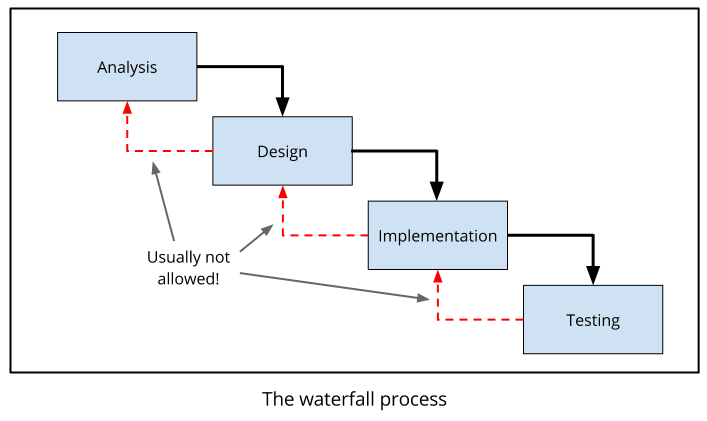
\includegraphics[width=\linewidth]{figs/process}\\
			\centering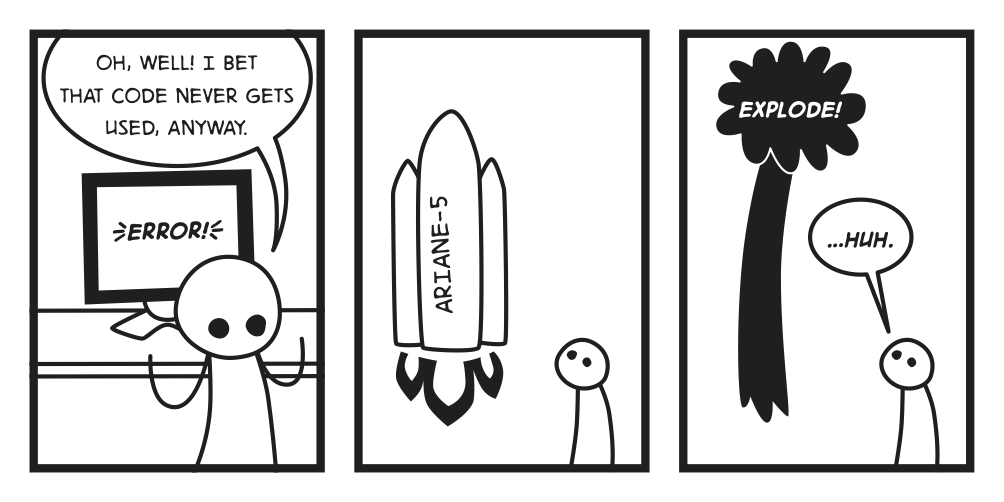
\includegraphics[width=\linewidth]{figs/ariane}\\
			\tiny{Source: \url{http://www.cosc.canterbury.ac.nz/csfieldguide/SoftwareEngineering.html}}
	\end{columns}
	\bigskip
	\scriptsize{More: \url{http://en.wikipedia.org/wiki/Iterative\_and\_incremental\_development}}
\end{frame}

\begin{frame}{Software engineering applied to videogames}{Software engineering (II)}
    %\begin{columns}
 	%   \column{.45\textwidth}
	Many development processes
	\begin{itemize}
		\item Usually, game development is \textbf{iterative}
  	\end{itemize}
	\bigskip
 	 %  \column{.55\textwidth}
			\centering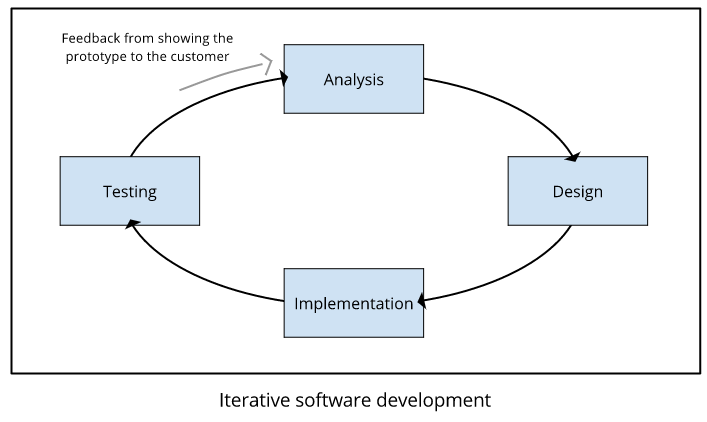
\includegraphics[width=0.58\linewidth]{figs/iterative}
			\centering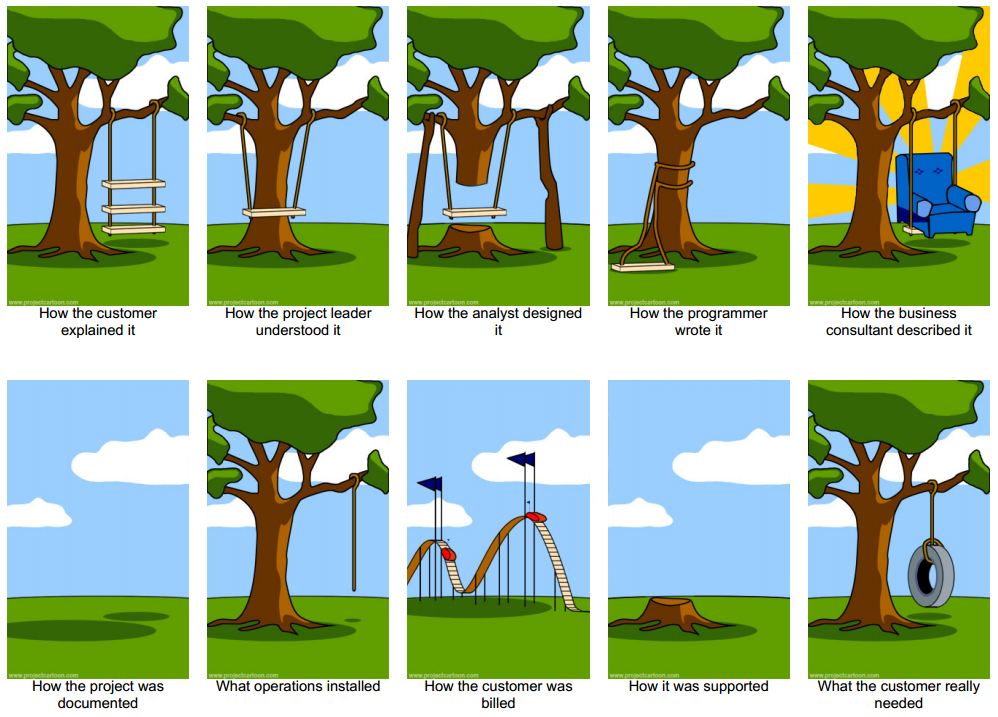
\includegraphics[width=0.48\linewidth]{figs/cartoon}\\
	%\end{columns}
	\normalsize{Design is critical for the videogame lifecycle: Class hierarchy}
\end{frame}

\subsection[Design pattern definition]{Design pattern definition}
\begin{frame}{Software engineering applied to videogames}{Design pattern definition (I)}
	Some problems happen frequently
	\begin{itemize}
		\item Experience is a valuable asset, but it is not enough
		\item A \alert{design pattern} stores knowledge on successful designs
  	\end{itemize}
	\begin{block}{Design pattern}
		It is the description of the communication among objects and classes customized to solve a generic design problem under a given context\\
		\scriptsize{\textit{Design Patterns. Elements of Reusable Object-Oriented Software}
		Erich Gamma, Richard Helm, Ralph Johnson, John Vlissides (GoF- Gang of Four), 2008}
	\end{block}
\end{frame}

\begin{frame}{Software engineering applied to videogames}{Design pattern definition (II)}
		Informal definition: A design pattern is a solution to a design problem
			\begin{itemize}
			\item Its utility has been verified by experience
			\item It must be reusable
			\end{itemize}	
	\centering\scriptsize{More: \url{http://en.wikipedia.org/wiki/Software\_design\_pattern}}
\end{frame}

\begin{frame}{Software engineering applied to videogames}{Design pattern definition (III)}
	Design patterns goals
	\begin{itemize}
		\item Provide a portfolio of reusable elements in software design
		\item Avoid loose time searching solutions to already solved problems
		\item Formalize a shared vocabulary
		\item Standarize designs
		\item Ease learning
 	\end{itemize}
	Design pattern do not want to
	\begin{itemize}
		\item Impose some design alternatives
		\item Remove designer creativity
	\end{itemize}
\end{frame}

\subsection[Design pattern structure]{Design pattern structure}
\begin{frame}{Software engineering applied to videogames}{Design pattern structure}
	Four components:
	\begin{enumerate}
		\item \textbf{Name}. Short name that identifies the pattern
		\item \textbf{Problem and context}. Problem that the pattern solves, context where it takes sense and list of \textit{preconditions}
		\item \textbf{Solution}. General solution not tied to any programming language. Usually described with UML diagrams.
		\item \textbf{Advantages/drawbacks}.
	\end{enumerate}
	Additionally:
	\begin{itemize}
		\item Classification, applicability, structure, roles, colaborators, implementation, example code, related patterns, ...
	\end{itemize}
\end{frame}

\section[Design patterns]{Design patterns}
\subsection[Types of design patterns]{Types of design patterns}
\begin{frame}{Design patterns}{Types of design patterns}
	Three great groups:
	\begin{enumerate}
		\item \textbf{Creational patterns}. Objects and data structures creation
			\begin{itemize}
			\item Singlenton, factory, abstract factory, ...
			\end{itemize}
		\item \textbf{Structural patterns}. Class hierarchy, relation and composition of objects
			\begin{itemize}
			\item Model-View-Controller (MVC), adapter, fa\c{c}ade, proxy, ...
			\end{itemize}
		\item \textbf{Behavioral patterns}. Objects message passing (communication)
			\begin{itemize}
			\item Observer, chain of responsability, command, iterator, state, strategy, ...
			\end{itemize}
	\end{enumerate}
	Additional domain patterns
	\begin{itemize}
		\item Web development, GUIs, business, ...
	\end{itemize}
\end{frame}

\subsection[Creational patterns]{Creational patterns}
\begin{frame}[plain]{Design patterns}{Creational patterns: Singlenton}
    \begin{columns}
 	   \column{.6\textwidth}
	   \begin{block}{Singlenton}
			\textbf{Problem}: Guarantee only one instance of a class\\
			\textbf{Solution}: Private constructor, instanciate the class through a public method\\
			\textbf{Example}: We need only one game instance\\
		\end{block}
 	   \column{.4\textwidth}
			\centering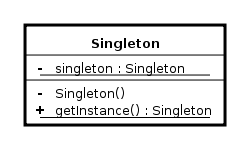
\includegraphics[width=\linewidth]{figs/singlenton}\\
\end{columns}
    \begin{block}{Code example}
	    \vspace{-0.2cm}
	    \lstinputlisting[language=java, basicstyle=\ttfamily\scriptsize]{code/Singleton.java}
		\vspace{-0.2cm}
	\end{block}
\end{frame}

\begin{frame}[plain]{Design patterns}{Creational patterns: Factory}
    \begin{columns}
 	   \column{.6\textwidth}
	   \begin{block}{Factory}
			\textbf{Problem}: Create new object\\
			\textbf{Solution}: Group object creation login in a factory class\\
			\textbf{Example}: Create warriors and rogues in a RPG game\\
		\end{block}
 	   \column{.4\textwidth}
			\centering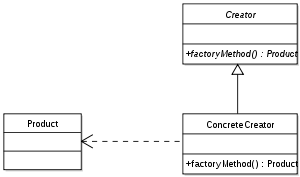
\includegraphics[width=\linewidth]{figs/factory}\\
	\end{columns}
	\begin{block}{Factory code example}
	    \vspace{-0.2cm}
	    \lstinputlisting[language=java, basicstyle=\ttfamily\scriptsize]{code/Factory.java}
		\vspace{-0.2cm}
	\end{block}
\end{frame}

\begin{frame}[plain]{Design patterns}{Creational patterns: Abstract factory (I)}
	   \begin{block}{Abstract factory}
			\textbf{Problem}: Create families of new objects\\
			\textbf{Solution}: Create a hierarchy of factories\\
			\textbf{Example}: Create human or orc warriors in a RPG game\\
		\end{block}
		\centering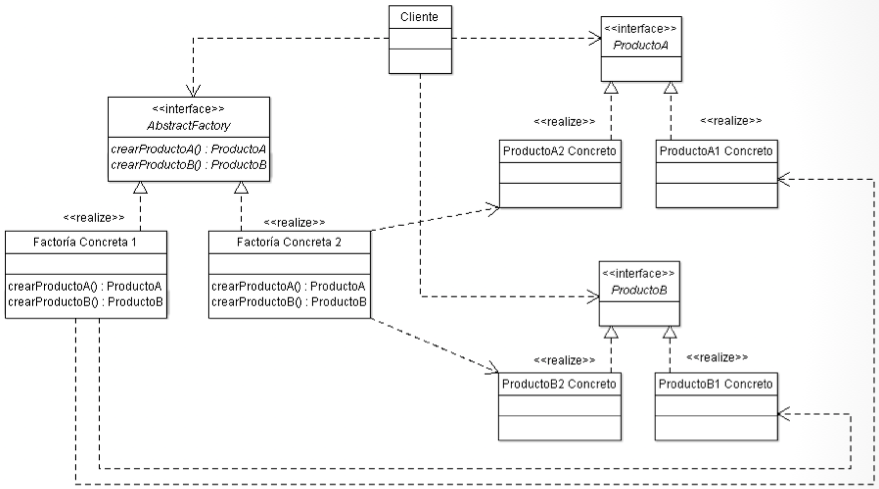
\includegraphics[width=0.8\linewidth]{figs/abstractfactory}\\
\end{frame}

\begin{frame}{Design patterns}{Creational patterns: Abstract factory (II)}
	\centering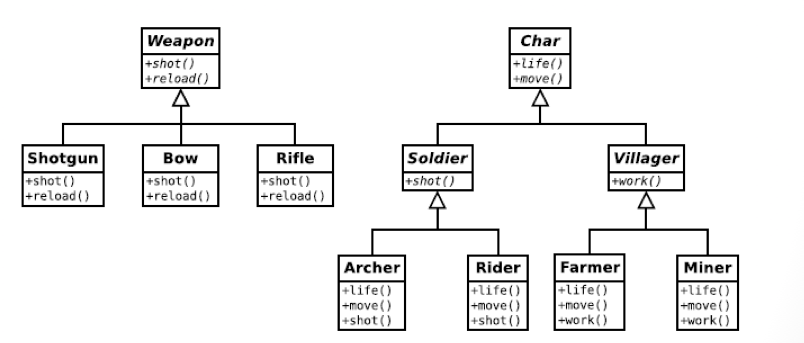
\includegraphics[width=0.8\linewidth]{figs/jerarquiajuego}\\
	\centering RTS game class hierarchy
\end{frame}

\begin{frame}{Design patterns}{Creational patterns: Abstract factory (III)}
	\centering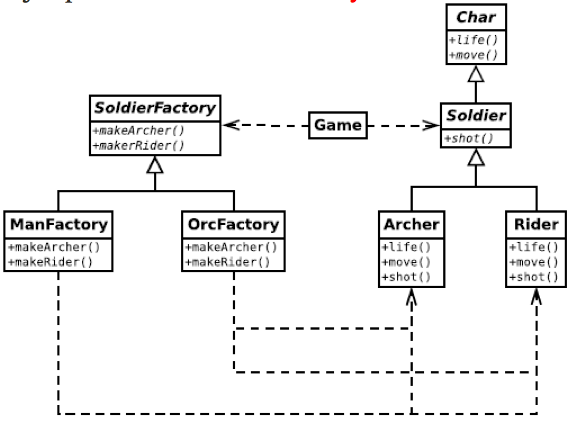
\includegraphics[width=0.7\linewidth]{figs/abstractfactorygame}\\
	\centering Example of \textit{abstract factory} applied to a RTS game
\end{frame}

\begin{frame}{Design patterns}{Creational patterns: Factory method}
    \begin{columns}
 	   \column{.5\textwidth}
	   \begin{block}{Factory Method}
			\textbf{Problem}: Create new objects\\
			\textbf{Solution}: Method that instanciates objects\\
			\textbf{Example}: Populate a village with characters\\
		\end{block}
 	   \column{.5\textwidth}
		\centering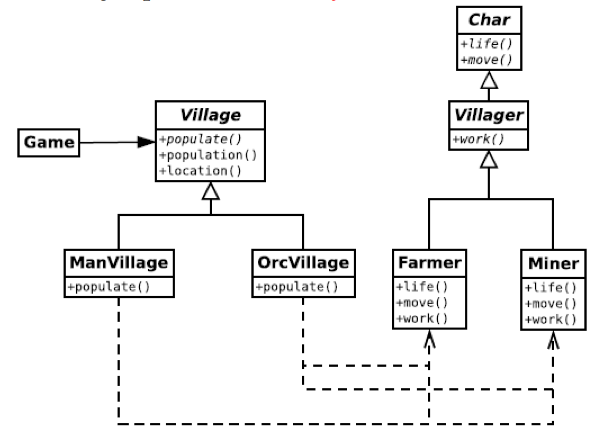
\includegraphics[width=\linewidth]{figs/factorymethod}\\
	\end{columns}
\end{frame}

\begin{frame}{Design patterns}{Creational patterns: Prototype}
	   \begin{block}{Prototype}
			\textbf{Problem}: Create a large number of objects whose instantiation is heavy\\
			\textbf{Solution}: Clone objects\\
			\textbf{Example}: Instanciate a large number of weapon objects\\
		\end{block}
		\centering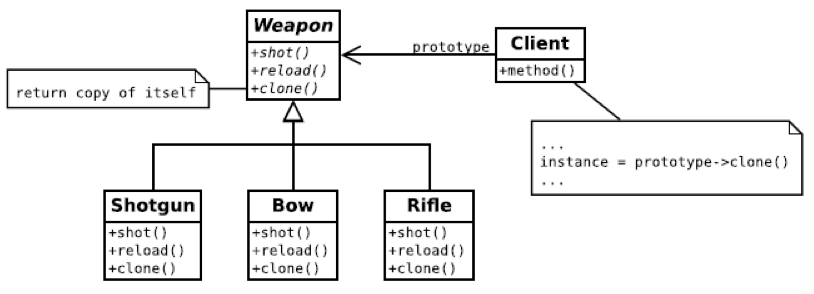
\includegraphics[width=0.9\linewidth]{figs/prototype}\\
\end{frame}

\subsection[Structural patterns]{Structural patterns}

\begin{frame}[plain]{Design patterns}{Structural patterns: MVC (I)}
    \begin{columns}
 	   \column{.6\textwidth}
	   \begin{block}{Model-View-Controller (MVC)}
			\textbf{Problem}: Decouple logic, data and visualization\\
			\textbf{Solution}: Use different classes to contain data, its visualization and the game control\\
			\textbf{Example}: Any game or graphical application\\
		\end{block}
 	   \column{.4\textwidth}
			\centering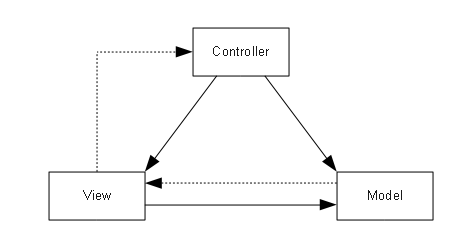
\includegraphics[width=\linewidth]{figs/mvc}\\
	\end{columns}
\end{frame}

\begin{frame}{Design patterns}{Structural patterns: MVC (II)}
	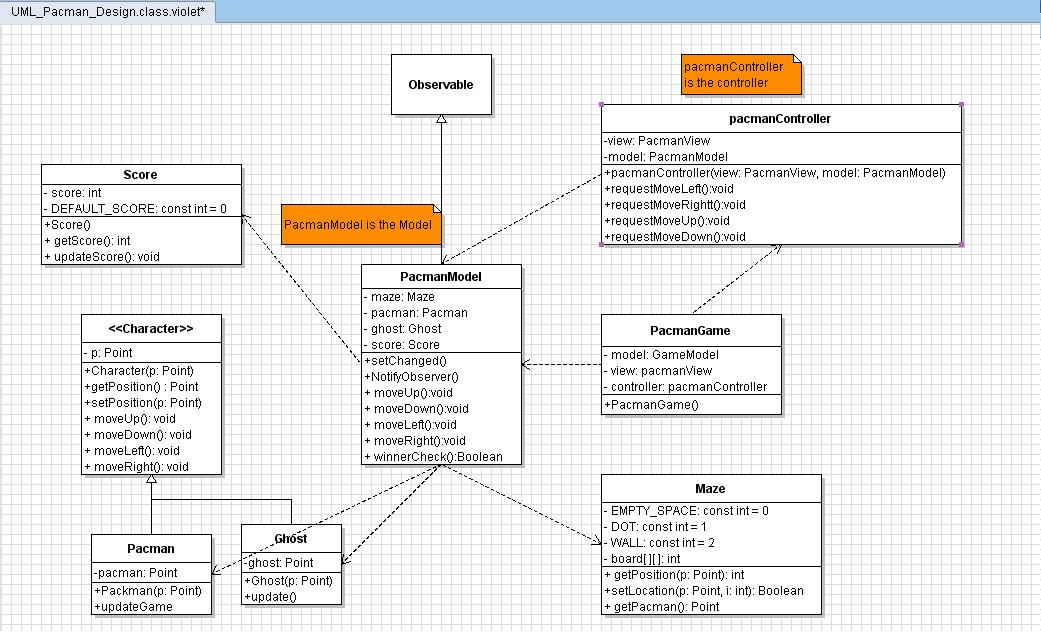
\includegraphics[width=0.9\linewidth]{figs/pacman}\\
	\centering \scriptsize{Source: \url{https://code.google.com/p/pacpounder/downloads/list}}
\end{frame}

\begin{frame}[plain]{Design patterns}{Structural patterns: MVC (III)}
	\centering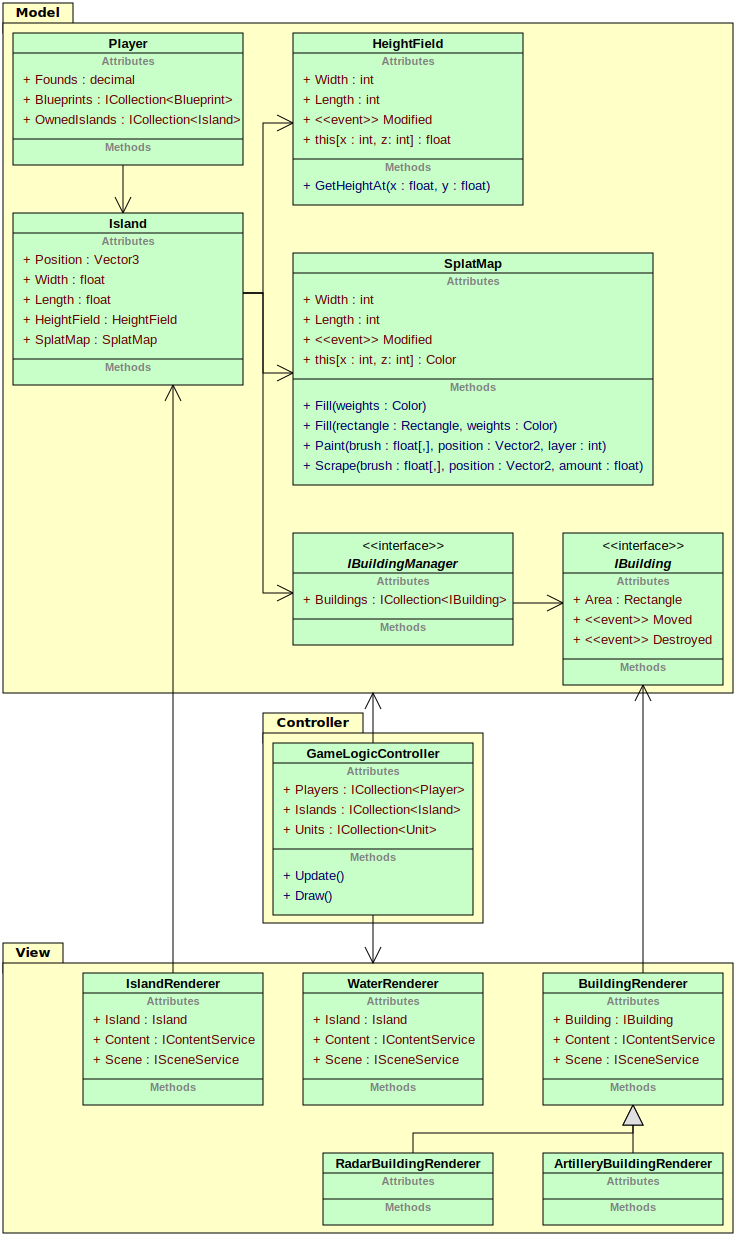
\includegraphics[width=0.4\linewidth]{figs/mvcgames}\\
	\centering \scriptsize{Source: \url{http://blog.nuclex-games.com/2010/09/mvc-in-games/}}
\end{frame}

\begin{frame}{Design patterns}{Structural patterns: Adapter}
    \begin{columns}
 	   \column{.6\textwidth}
	   \begin{block}{Adapter}
			\textbf{Problem}: One class needs to invoke a method in another class, but it cannot\\
			\textbf{Solution}: Use an intermediate class with a new interface\\
			\textbf{Example}: Incompatible third-party library\\
		\end{block}
 	   \column{.4\textwidth}
			\centering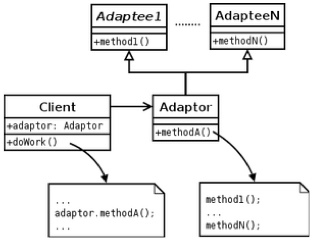
\includegraphics[width=\linewidth]{figs/adapter}\\
	\end{columns}
\end{frame}

\begin{frame}{Design patterns}{Structural patterns: Composite}
    \begin{columns}
 	   \column{.6\textwidth}
	   \begin{block}{Composite}
			\textbf{Problem}: Store objects that might contain other objects\\
			\textbf{Solution}: Objects composition\\
			\textbf{Example}: Game whose player keeps an inventory whose items might contain other items\\
		\end{block}
 	   \column{.4\textwidth}
			\centering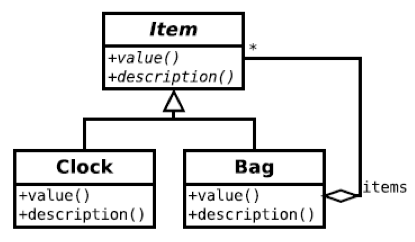
\includegraphics[width=\linewidth]{figs/composite}
	\end{columns}
\end{frame}

\begin{frame}{Design patterns}{Structural patterns: Fa\c{c}ade}
    \begin{columns}
 	   \column{.5\textwidth}
	   \begin{block}{Fa\c{c}ade}
			\textbf{Problem}: Complex interface to a set of classes\\
			\textbf{Solution}: Create an intermediate class that simplifies the interface\\
			\textbf{Example}: Graphical library with several operation modes\\
		\end{block}
 	   \column{.5\textwidth}
			\centering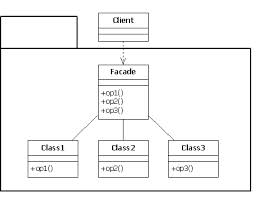
\includegraphics[width=\linewidth]{figs/facade.jpeg}
	\end{columns}
\end{frame}

\subsection[Behavioral patterns]{Behavioral patterns}

\begin{frame}{Design patterns}{Behavioral patterns: Observer (I)}
	   \begin{block}{Observer}
			\textbf{Problem}: Notify a set of objects when another object changes\\
			\textbf{Solution}: Link a set of observers to an observed object\\
			\textbf{Example}: A view that has to know when the model changes\\
		\end{block}
		\bigskip
		\centering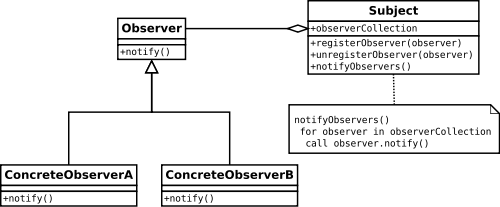
\includegraphics[width=0.7\linewidth]{figs/observer}
\end{frame}

\begin{frame}[plain]{Design patterns}{Behavioral patterns: Observer (II)}
	\centering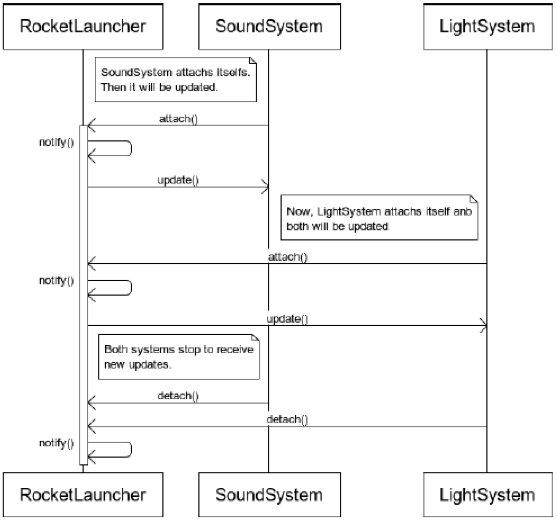
\includegraphics[width=0.6\linewidth]{figs/observergame}
\end{frame}

\begin{frame}{Design patterns}{Behavioral patterns: Observer (III)}
	\vspace{-0.3cm}
    \begin{block}{DataStore.java}
	    \vspace{-0.2cm}
	    \lstinputlisting[language=java, basicstyle=\ttfamily\scriptsize]{code/DataStore.java}
		\vspace{-0.2cm}
	\end{block}

	\vspace{-0.2cm}
    \begin{block}{Screen.java}
	    \vspace{-0.2cm}
	    \lstinputlisting[language=java, basicstyle=\ttfamily\scriptsize]{code/Screen.java}
		\vspace{-0.3cm}
	\end{block}
\end{frame}

\begin{frame}{Design patterns}{Behavioral patterns: Strategy (I)}
	   \begin{block}{Observer}
			\textbf{Problem}: Choose in execution time which method use from several ones\\
			\textbf{Solution}: Encapsulate the method in a class\\
			\textbf{Example}: A fighter with several fighting styles\\
		\end{block}
		\bigskip
		\centering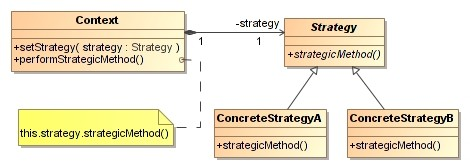
\includegraphics[width=0.7\linewidth]{figs/strategy}
\end{frame}

\begin{frame}[plain]{Design patterns}{Behavioral patterns: Stategy (II)}
	\centering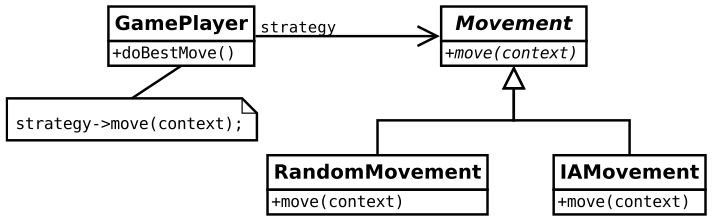
\includegraphics[width=0.8\linewidth]{figs/strategygame}
\end{frame}

\begin{frame}{Design patterns}{Behavioral patterns: State (I)}
    \begin{columns}
 	   \column{.5\textwidth}
	   \begin{block}{State}
			\textbf{Problem}: Implement a state machine\\
			\textbf{Solution}: Encapsulate state transitions\\
			\textbf{Example}: NPC behavior\\
		\end{block}
 	   \column{.5\textwidth}
			\centering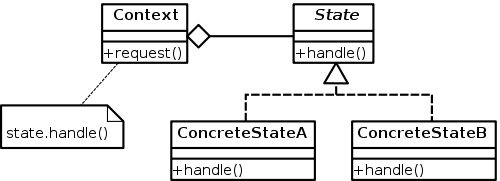
\includegraphics[width=\linewidth]{figs/state}\\
	\end{columns}
\end{frame}

\begin{frame}{Design patterns}{Behavioral patterns: State (II)}
			\centering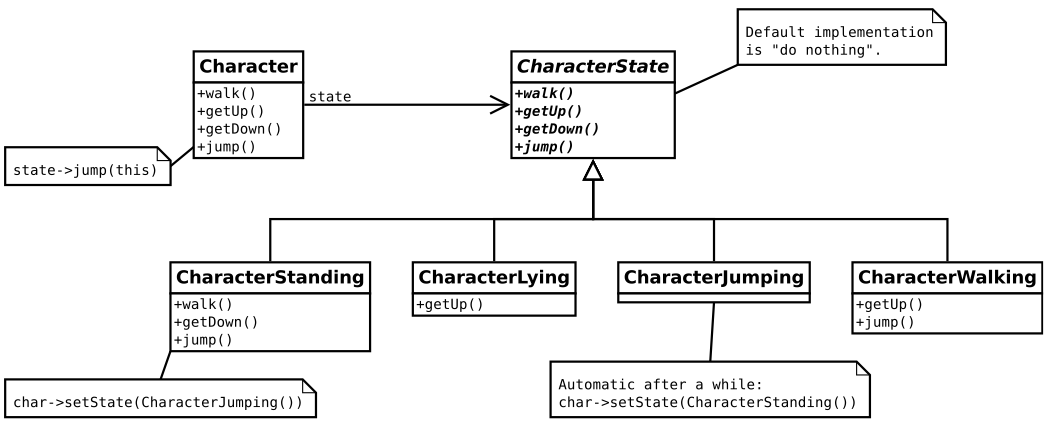
\includegraphics[width=\linewidth]{figs/stategame}
\end{frame}

\begin{frame}{Design patterns}{Behavioral patterns: Template method (I)}
    \begin{columns}
 	   \column{.5\textwidth}
	   \begin{block}{Template Method}
			\textbf{Problem}: Customize an algorithm\\
			\textbf{Solution}: Divide the algorithm in methods that can be overriden\\
			\textbf{Example}: Chess and checkers games\\
		\end{block}
 	   \column{.5\textwidth}
			\centering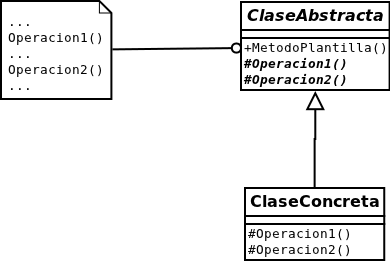
\includegraphics[width=0.8\linewidth]{figs/template}\\
	\end{columns}
\end{frame}

\begin{frame}{Design patterns}{Behavioral patterns: Template method (II)}
			\centering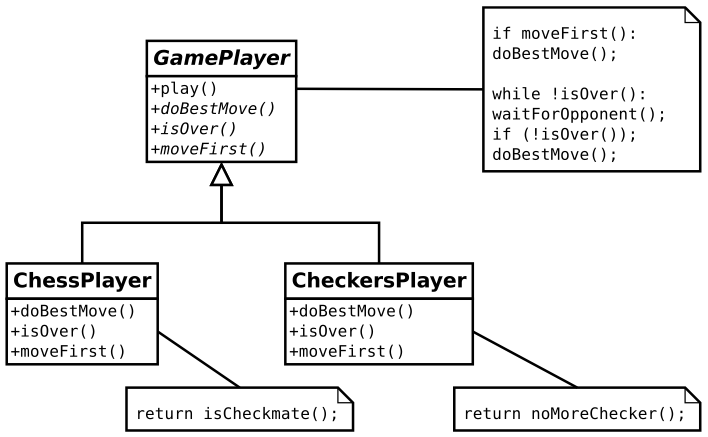
\includegraphics[width=0.6\linewidth]{figs/templategame}
\end{frame}

\section{Videogame models}
\subsection{Render loop}
\begin{frame}{Videogame models}{Render loop (I)}
    \begin{columns}
 	   \column{.5\textwidth}
		\begin{itemize}
	   	\item The render loop handles visualization and rendering
	   	\item Objectives in 2D games
		\begin{itemize}
			\item Minimize pixels to draw: Draw only those pixels that have changed
			\item Maximize fps
		\end{itemize}
		\end{itemize}
 	   \column{.5\textwidth}
	\centering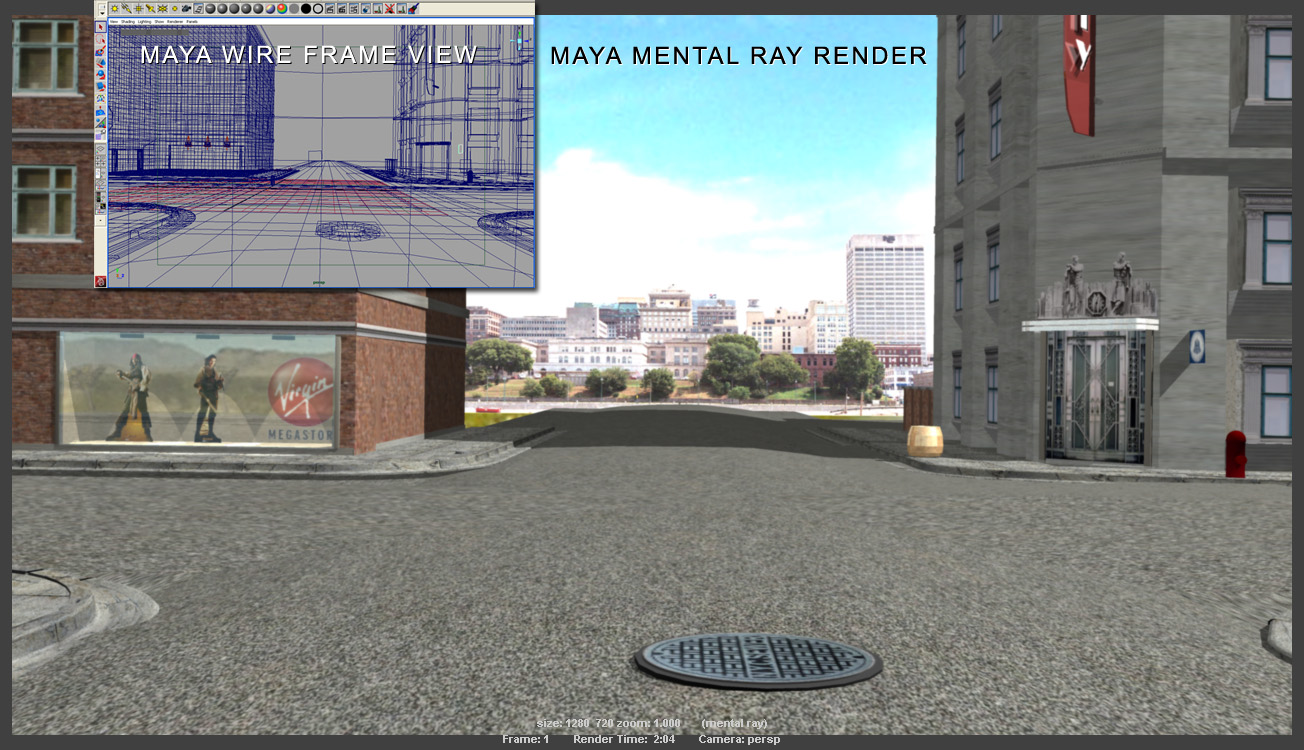
\includegraphics[width=0.8\linewidth]{figs/rendering}\\
	Render example
 	\end{columns}
	\begin{itemize}
	\item Objectives in 3D games
		\begin{itemize}
			\item Camera uses to change everytime: The same technique cannot be used
			\item Minimize the number of primites to draw in each iteration of the render loop
		\end{itemize}
	\end{itemize}
\end{frame}

\begin{frame}{Videogame models}{Render loop (II)}
	    \vspace{-0.2cm}
    \begin{block}{Render loop}
	    \vspace{-0.2cm}
	    \lstinputlisting[language=java, basicstyle=\ttfamily\scriptsize]{code/renderloop.java}
		\vspace{-0.2cm}
	\end{block}
	Info: \url{http://wiki.wxwidgets.org/Making\_a\_render\_loop}
\end{frame}


\subsection{Game loop}
\begin{frame}{Videogame models}{Game loop (I)}
	   	The main element in a videogame is the \alert{game loop}
		\begin{itemize}
			\item It is the main control structure in the game
			\item It controls its execution
			\item It handlers the transitions among states
			\item The game loop independizes the game execution from the hardware
		\end{itemize}
		Classical programs only reacts with user actions
		\begin{itemize}
			\item Videogames are always performing an action
			\item Game loop implements this easely
			\item The game engine contains the game loop
		\end{itemize}
\end{frame}

\begin{frame}{Videogame models}{Game loop (II)}
		\begin{itemize}
		   	\item There are many subsystems in a videogame
			\begin{itemize}
				\item Rendering engine (render is to generate an image)
				\item Collition detection
				\item Collition handling
				\item AI subsystem
					\item Game subsystem
			\end{itemize}
			\item Most of these subsystems require periodic updates
			\item The most critical one is the animation system
			\begin{itemize}
				\item Frequency: 30 or 60 Hz
				\item Syncronized with the rendering subsystem
				\item Objective: Provide a good fps rate to generate a realistic experience
			\end{itemize}
			\item Not all the components are so strict, for instance, AI
		\end{itemize}
\end{frame}

\begin{frame}{Videogame models}{Game loop (III)}
	\begin{itemize}
	   	\item There are several ways to implement the game loop
	   	\item The easiest one is to have several loops within the game loop
		\begin{itemize}
			\item Render loop
			\item AI loop
			\item Multimedia loop
			\item Iteration loop
		\end{itemize}
	\end{itemize}

    \begin{columns}
 	   \column{.4\textwidth}
    \begin{block}{Basic game loop}
	    \vspace{-0.2cm}
	    \lstinputlisting[language=java, basicstyle=\ttfamily\scriptsize]{code/gameloop1.java}
		\vspace{-0.2cm}
	\end{block}
   \column{.6\textwidth}
    \begin{block}{Game loop}
	    \vspace{-0.2cm}
	    \lstinputlisting[language=java, basicstyle=\ttfamily\scriptsize]{code/gameloop2.java}
		\vspace{-0.2cm}
	\end{block}
	\end{columns}
\end{frame}

\begin{frame}{Videogame models}{Game loop (IV)}
	    \vspace{-0.3cm}
    \begin{columns}
 	   \column{.7\textwidth}
    \begin{block}{}
	    \vspace{-0.2cm}
	    \lstinputlisting[language=c, basicstyle=\ttfamily\scriptsize]{code/pong.c}
		\vspace{-0.2cm}
	\end{block}
   \column{.3\textwidth}
   	Pong game loop example
	\centering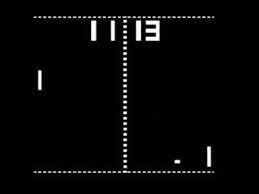
\includegraphics[width=\linewidth]{figs/pong.jpeg}
	\end{columns}
\end{frame}

\begin{frame}[plain]{Videogame models}{Game loop (V)}
	\centering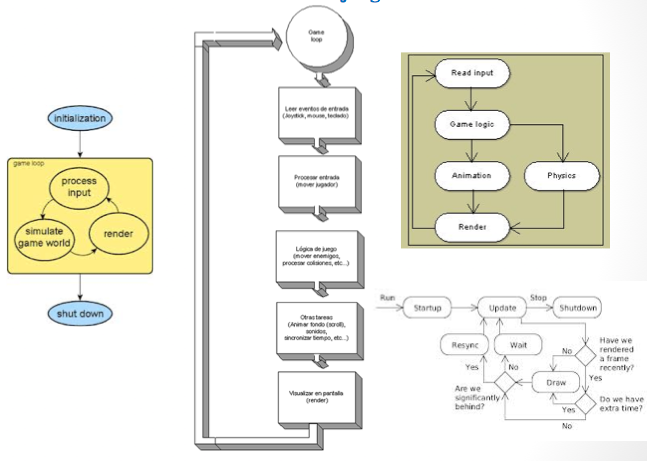
\includegraphics[width=\linewidth]{figs/gameloops}
\end{frame}

\begin{frame}{Videogame models}{Game loop (VI)}
	    The game loop depends on the platform
		\begin{itemize}
			\item DOS games and some consoles are designed to exploit computational resources
			\item PC games depend on limitations imposed by the OS
			\item Games use to be multithreaded to exploit multicore machines
		\end{itemize}
\end{frame}

\section{Game architectures}
\subsection{Game architectures}

\begin{frame}{Game architectures}{Game architectures}
    Game loop can be implemented in different ways
	\begin{itemize}
		\item Architectures based on callbacks
		\item Architectures based on events
		\item Architectures based on state machines
	\end{itemize}
	Most of them implement one or more control loops
\end{frame}

\subsection{Callbacks}
\begin{frame}{Game architectures}{Callbacks (I)}
	\begin{itemize}
		\item \textbf{Callbacks}: Code that is executed to handle an event
		\begin{itemize}
			\item Function or object
			\item Callbacks are used to ``fill'' source code
		\end{itemize}
		\item Related term: \textbf{framework}
		\begin{itemize}
			\item Application partially completed that the developer has to complete
		\end{itemize}
	\end{itemize}
\end{frame}

\begin{frame}{Videogame models}{Callbacks (II)}
	\vspace{-0.3cm}
    \begin{columns}
 	   	\column{.9\textwidth}
    		\begin{block}{}
	    	\vspace{-0.2cm}
	    	\lstinputlisting[language=c, basicstyle=\ttfamily\scriptsize]{code/callback.c}
			\vspace{-0.2cm}
			\end{block}
	\end{columns}
\end{frame}

\subsection{Events}
\begin{frame}{Game architectures}{Events}
	\begin{itemize}
		\item An event represents a change in the game state
		\item Two types
		\begin{itemize}
			\item \textbf{External}: Generated by the interactions\\Example, The player press a key or moves the joystick
			\item \textbf{Internal}: Generated by the game logic\\Example, NPC respawn
		\end{itemize}
		\item Most game engines include an event subsystem
		\begin{itemize}
			\item Closely related to the \textit{Observer} pattern
		\end{itemize}

	\end{itemize}
\end{frame}

\subsection{State machine}
\begin{frame}{Game architectures}{State machine}
	\vspace{-0.3cm}
	A game goes through a number of \alert{states}
		\begin{itemize}
			\item Introduction
			\item Main menu
			\item Game
			\item Game over
		\end{itemize}
	\textbf{State machine}: A set of states and transitions
	\vspace{0.3cm}
	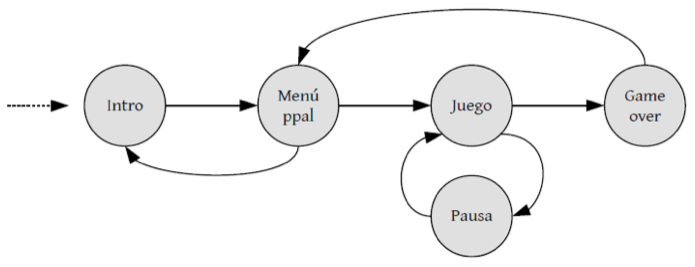
\includegraphics[width=0.7\linewidth]{figs/states}\\
	\vspace{-0.2cm}
	Warning: State machines play a mayor role in game AI
\end{frame}



\end{document}
